\chapter{Wprowadzenie} \label{ch:wprowadzenie}

Choroba Parkinsona (ang. \emph {Parkinson Disease, PD}) to zwyrodnieniowe schorzenie mózgu, które wiąże się z objawami ruchowymi, takimi jak spowolnienie ruchowe,
drżenie, sztywność oraz zaburzenia chodu i równowagi.
Ponadto może prowadzić do różnorodnych powikłań niemotorycznych, obejmujących zaburzenia poznawcze, stany psychiczne,
trudności ze snem oraz dolegliwości sensoryczne, w tym ból.
Początkowe objawy często rozwijają się stopniowo, nasilając się w miarę upływu czasu.
Postęp choroby prowadzi do znacznego stopnia niepełnosprawności, co może wymagać wsparcia i opieki.
U wielu osób zdiagnozowanych z chorobą Parkinsona występują także zmiany w sferze psychicznej i behawioralnej, takie jak
trudności ze snem, depresja, problemy z pamięcią oraz uczucie przewlekłego zmęczenia.

\begin{figure}[htbp]
	\centering
	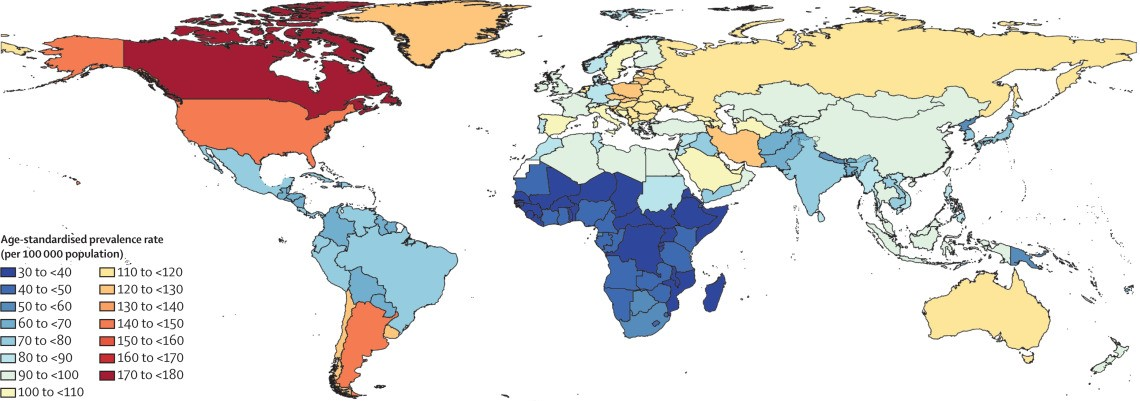
\includegraphics[width=0.9\textwidth]{./img/map}
	\caption{Choroba Parkinsona na świecie \cite{global_PD}}
    \label{fig:PD_map}
\end{figure}

Zgodnie z danymi przedstawionymi w raporcie Światowej Organizacji Zdrowia \cite{WHO}, choroba Parkinsona (PD) stanowi obecnie narastający problem na skalę światową. Zarówno wskaźniki niepełnosprawności, jak i zgony związane z tą chorobą rosną szybciej niż w przypadku innych zaburzeń neurologicznych.

W ciągu ostatnich 25 lat zaobserwowano podwojenie częstości występowania PD na całym świecie.
Globalne szacunki na rok 2019 wskazują, że liczba osób cierpiących na PD przekroczyła 8,5 miliona, co oznacza wzrost o 81\% w porównaniu z danymi z roku 2000.
Jednocześnie liczba zgonów związanych z PD wyniosła 329 000, co stanowi wzrost o ponad 100\% w porównaniu z rokiem 2000 \cite{global_PD}.
W Polsce z chorobą Parkinsona zmaga się około 100 tys. pacjentów, z czego około 20\% jest już w stadium zaawansowanym
według informacji przekazywanych przez Fundację Chorób Mózgu.
Ponadto co roku w naszym kraju wykrywanych jest ok. 8 tys. nowych zachorowań.

PD jest istotną sprawą dotyczącą zdrowia publicznego, ponieważ jej częstotliwość występowania związana jest ze zjawiskiem starzejącego się społeczeństwa.
Razem z innymi chorobami neurodegeneracyjnymi, takimi jak choroba Alzheimera, ma szanse stać się drugą zaraz za nowotworami przyczyną zgonów do 2040 roku (WHO).

Przyczyna PD nie jest znana, ale uważa się, że powstaje w wyniku złożonej interakcji pomiędzy czynnikami genetycznymi i
narażeniem na czynniki środowiskowe, takie jak pestycydy, rozpuszczalniki i zanieczyszczenia powietrza.
Niektóre przypadki wydają się dziedziczne, a kilka można przypisać określonym wariantom genetycznym.
Chociaż uważa się, że genetyka odgrywa rolę w chorobie Parkinsona, w większości przypadków choroba nie występuje rodzinnie \cite{National_Institute_on_Aging_2022}.

\begin{figure}[htbp]
	\centering
	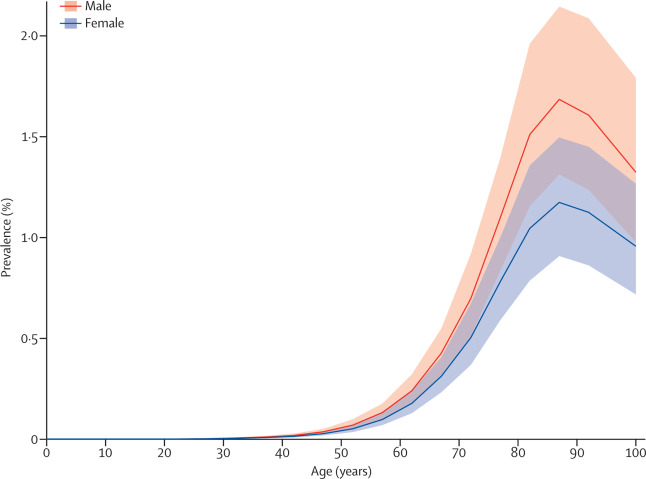
\includegraphics[width=0.5\textwidth]{./img/PD_prevalence}
	\caption{Rozpowszechnienie choroby Parkinsona w zależności od wieku \cite{global_PD}}
    \label{fig:PD_prevalance}
\end{figure}

Mimo że każdy może być narażony na ryzyko rozwoju tej choroby, to częściej występuje ona u mężczyzn niż u kobiet,
a wiek stanowi kluczowy element wpływający na ryzyko zachorowania, co można zobaczyć na Rys.\ref{fig:PD_prevalance}.
Statystyki pokazują, że ryzyko zachorowania rośnie wraz z wiekiem, chociaż choroba może dotyczyć także młodszych osób (nawet w wieku 20 lat).
U większości pacjentów po raz pierwszy choroba rozwija się po 60 roku życia, około 5\% do 10\% doświadcza jej początku przed 50 rokiem życia.
Postacie choroby Parkinsona o wczesnym początku są często, choć nie zawsze, dziedziczne i niektóre formy zostały powiązane z
określonymi zmianami w genach \cite{National_Institute_on_Aging_2022}.

Proces diagnozowania choroby jest niezwykle złożony i czasochłonny, nie istnieje obecnie pojedyncze badanie pozwalające na postawienie diagnozy.
W związku z tym poszukuje się nowych rozwiązań, które mogłyby usprawnić ten proces.
Coraz częściej wykorzystuje się metody uczenia maszynowego i sztucznej inteligencji w dziedzinie medycyny.
W niniejszej pracy analizowany jest aktualny stan rzeczy oraz przedstawiane jest proponowane rozwiązanie, dotyczące automatycznej diagnostyki
choroby Parkinsona na podstawie głosu.

%---------------------------------------------------------------------------

\section{Cel pracy}
\label{sec:celPracy}

Celem pracy jest detekcja choroby Parkinsona na podstawie sygnału głosowego z wykorzystaniem metod uczenia maszynowego.
Obejmuje to dokładny przegląd literaturowy ze szczególnym uwzględnieniem aktualnie najlepszych algorytmów
dostępnych w literaturze.
Pośrednim celem jest ocena skuteczności wybranych architektur konwolucyjnych sieci neuronowych (CNN) oraz analiza, która z wypowiadanych przez
pacjentów samogłosek niesie ze sobą najwięcej informacji diagnostycznej.

%---------------------------------------------------------------------------

\section{Zakres pracy}
\label{sec:zakresPracy}
